%%%%%%%%%%%%%%%%%%%%%%%%%%%%%%%%%%%%%%%%%
% Programming/Coding Assignment
% LaTeX Template
%
% This template has been downloaded from:
% http://www.latextemplates.com
%
% Original author:
% Ted Pavlic (http://www.tedpavlic.com)
%
% Note:
% The \lipsum[#] commands throughout this template generate dummy text
% to fill the template out. These commands should all be removed when 
% writing assignment content.
%
% This template uses a Perl script as an example snippet of code, most other
% languages are also usable. Configure them in the "CODE INCLUSION 
% CONFIGURATION" section.
%
%%%%%%%%%%%%%%%%%%%%%%%%%%%%%%%%%%%%%%%%%

%----------------------------------------------------------------------------------------
%	PACKAGES AND OTHER DOCUMENT CONFIGURATIONS
%----------------------------------------------------------------------------------------

\documentclass{article}

\usepackage{fancyhdr} % Required for custom headers
\usepackage{lastpage} % Required to determine the last page for the footer
\usepackage{extramarks} % Required for headers and footers
\usepackage[usenames,dvipsnames]{color} % Required for custom colors
\usepackage{graphicx} % Required to insert images
\usepackage{subcaption}
\usepackage{listings} % Required for insertion of code
\usepackage{courier} % Required for the courier font
\usepackage{amsmath}
\usepackage{framed}

% Margins
\topmargin=-0.45in
\evensidemargin=0in
\oddsidemargin=0in
\textwidth=6.5in
\textheight=9.0in
\headsep=0.25in

\linespread{1.1} % Line spacing

% Set up the header and footer
\pagestyle{fancy}
\lhead{\hmwkAuthorName} % Top left header
\chead{\hmwkClass\ (\hmwkClassTime): \hmwkTitle} % Top center head
%\rhead{\firstxmark} % Top right header
\lfoot{\lastxmark} % Bottom left footer
\cfoot{} % Bottom center footer
\rfoot{Page\ \thepage\ of\ \protect\pageref{LastPage}} % Bottom right footer
\renewcommand\headrulewidth{0.4pt} % Size of the header rule
\renewcommand\footrulewidth{0.4pt} % Size of the footer rule

\setlength\parindent{0pt} % Removes all indentation from paragraphs

%----------------------------------------------------------------------------------------
%	CODE INCLUSION CONFIGURATION
%----------------------------------------------------------------------------------------

\definecolor{mygreen}{rgb}{0,0.6,0}
\definecolor{mygray}{rgb}{0.5,0.5,0.5}
\definecolor{mymauve}{rgb}{0.58,0,0.82}

\lstset{ %
  backgroundcolor=\color{white},   % choose the background color
  basicstyle=\footnotesize,        % size of fonts used for the code
  breaklines=true,                 % automatic line breaking only at whitespace
  captionpos=b,                    % sets the caption-position to bottom
  commentstyle=\color{mygreen},    % comment style
  escapeinside={\%*}{*)},          % if you want to add LaTeX within your code
  keywordstyle=\color{blue},       % keyword style
  stringstyle=\color{mymauve},     % string literal style
}

%----------------------------------------------------------------------------------------
%	DOCUMENT STRUCTURE COMMANDS
%	Skip this unless you know what you're doing
%----------------------------------------------------------------------------------------

% Header and footer for when a page split occurs within a problem environment
\newcommand{\enterProblemHeader}[1]{
%\nobreak\extramarks{#1}{#1 continued on next page\ldots}\nobreak
%\nobreak\extramarks{#1 (continued)}{#1 continued on next page\ldots}\nobreak
}

% Header and footer for when a page split occurs between problem environments
\newcommand{\exitProblemHeader}[1]{
%\nobreak\extramarks{#1 (continued)}{#1 continued on next page\ldots}\nobreak
%\nobreak\extramarks{#1}{}\nobreak
}

\setcounter{secnumdepth}{0} % Removes default section numbers
\newcounter{homeworkProblemCounter} % Creates a counter to keep track of the number of problems
\setcounter{homeworkProblemCounter}{0}

\newcommand{\homeworkProblemName}{}
\newenvironment{homeworkProblem}[1][Problem \arabic{homeworkProblemCounter}]{ % Makes a new environment called homeworkProblem which takes 1 argument (custom name) but the default is "Problem #"
\stepcounter{homeworkProblemCounter} % Increase counter for number of problems
\renewcommand{\homeworkProblemName}{#1} % Assign \homeworkProblemName the name of the problem
\section{\homeworkProblemName} % Make a section in the document with the custom problem count
\enterProblemHeader{\homeworkProblemName} % Header and footer within the environment
}{
\exitProblemHeader{\homeworkProblemName} % Header and footer after the environment
}

\newcommand{\problemAnswer}[1]{ % Defines the problem answer command with the content as the only argument
\noindent\framebox[\columnwidth][c]{\begin{minipage}{0.98\columnwidth}#1\end{minipage}} % Makes the box around the problem answer and puts the content inside
}

\newcommand{\homeworkSectionName}{}
\newenvironment{homeworkSection}[1]{ % New environment for sections within homework problems, takes 1 argument - the name of the section
\renewcommand{\homeworkSectionName}{#1} % Assign \homeworkSectionName to the name of the section from the environment argument
\subsection{\homeworkSectionName} % Make a subsection with the custom name of the subsection
\enterProblemHeader{\homeworkProblemName\ [\homeworkSectionName]} % Header and footer within the environment
}{
\enterProblemHeader{\homeworkProblemName} % Header and footer after the environment
}

%----------------------------------------------------------------------------------------
%	NAME AND CLASS SECTION
%----------------------------------------------------------------------------------------

\newcommand{\hmwkTitle}{Assignment 3} % Assignment title
\newcommand{\hmwkDueDate}{Friday, Mar. 19, 2018} % Due date
\newcommand{\hmwkClass}{CSC411} % Course/class
\newcommand{\hmwkClassTime}{LEC 5101/0101} % Class/lecture time
\newcommand{\hmwkAuthorName}{Zhongtian Ouyang/Yihao Ni} % Your name

%----------------------------------------------------------------------------------------
%	TITLE PAGE
%----------------------------------------------------------------------------------------

\title{
\vspace{2in}
\textmd{\textbf{\hmwkClass:\ \hmwkTitle}}\\
\normalsize\vspace{0.1in}\small{Due\ on\ \hmwkDueDate}\\
\vspace{0.1in}
\vspace{3in}
}

\author{\textbf{\hmwkAuthorName}}
\date{} % Insert date here if you want it to appear below your name

%----------------------------------------------------------------------------------------

\begin{document}

\maketitle
\clearpage
%----------------------------------------------------------------------------------------
%	PROBLEM 1
%----------------------------------------------------------------------------------------

% To have just one problem per page, simply put a \clearpage after each problem

\begin{homeworkProblem}
\noindent \textit{Useful keywords}\\
This dataset contains headlines with the word "trump", there are 1968 real news and 1268 fake news, with 4814 different words in those headlines. 

We choose "korea", "black" and "ban" to predict whether a news is real or fake. The following output is obtained by running part1() in fake.py.
\begin{framed}
Word "korea" appears 4.522\% in real news and 0.000\% in fake news.\\
Word "black" appears 0.051\% in real news and 3.236\% in fake news.\\
Word "ban" appears 5.335\% in real news and 1.464\% in fake news.
\end{framed}

From the output we can say that a news containing "korea" and "ban" is more likely to be a real news, while a news containing "black" is more likely to be a fake news.

\end{homeworkProblem}
\clearpage
%----------------------------------------------------------------------------------------
%	PROBLEM 2
%----------------------------------------------------------------------------------------

\begin{homeworkProblem}
\noindent \textit{Neural network}\\

\end{homeworkProblem}
\clearpage

%----------------------------------------------------------------------------------------
%	PROBLEM 3
%----------------------------------------------------------------------------------------

\begin{homeworkProblem}
\noindent \textit{Compute the gradient}

\begin{framed}
\begin{lstlisting}[language=python]

\end{lstlisting}
\end{framed}

\end{homeworkProblem}
\clearpage
%----------------------------------------------------------------------------------------
%	PROBLEM 4
%----------------------------------------------------------------------------------------

\begin{homeworkProblem}
\noindent \textit{Training a logistic regression model}\\

We train the logistic regression model by pytorch using a linear model and a cross entropy loss. Weight\_decay in optimizer is chosen to be $5*10^{-3}$. The value is larger the better. But with a larger value than our choice, theta may not be trained to a suitable value, lowering the validation set performance.\\~\\
Following is the learning curves (performance vs. iteration) of the Logistic Regression model. 

\begin{figure}[!ht]
\centering
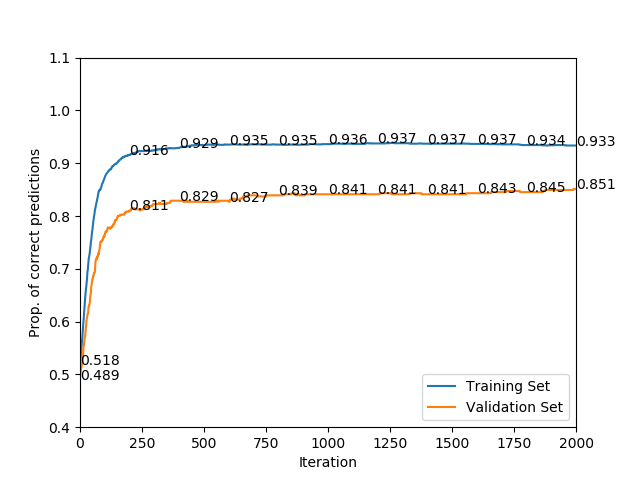
\includegraphics[width=1\linewidth]{p4.png}
\caption{performance}
\label{fig:p4w}
\end{figure}

The model performs fairly well after only several iterations, and the validation performance reaches its max at about 2000 iterations (tried more iterations but more iterations will lead to a poorer validation performance). The test performance under this model is as follows:
\begin{framed}
Test Set performance : 0.8326530612244898
\end{framed}

\end{homeworkProblem}
\clearpage

%----------------------------------------------------------------------------------------
%	PROBLEM 5
%----------------------------------------------------------------------------------------

\begin{homeworkProblem}
\noindent \textit{Formulation}\\

For logistic regression, $\theta_k$ is the weight of the kth keyword, if the weight is positive, then the a piece of news containing the kth keyword is more likely to be a real news, and vice versa. $I_k(x)$ is whether or not the keyword presents, 1 for presence and 0 for not. If the output is greater than a given threshold, we say the news is real, and if less than the threshold, we say the news is fake.

For naive bayes, $\theta_0$ is the default weight, that is to say, it indicates whether the news is real or fake when there is no words in the headline. $\theta_k$ is the weight for the kth keyword. $I_k(x)$ is again whether or not the keyword presents, 1 for presence and 0 for not. If the output is greater than a given threshold, we say the news is real, and if less than the threshold, we say the news is fake.

\end{homeworkProblem}
\clearpage
%----------------------------------------------------------------------------------------
%	PROBLEM 6
%----------------------------------------------------------------------------------------
\begin{homeworkProblem}
\noindent \textit{Words obtained using Logistic Regression}

For this problem, we get the value of theta by substracting the weight for the news to be fake from the weight for the news to be real given the presence of a keyword. This works as if the result is larger, the news is more likely to be real than fake, and vice versa.
\subsection{Part(a)}
\begin{framed}
\begin{lstlisting}[language=python]
========================== Part 6a ==========================
TOP 10 positive thetas with stop words: 
	1 : "ban"   with theta 0.2616
	2 : "scaramucci"   with theta 0.2545
	3 : "donald"   with theta 0.2479
	4 : "refugee"   with theta 0.2459
	5 : "us"   with theta 0.2443
	6 : "call"   with theta 0.2384
	7 : "climate"   with theta 0.2372
	8 : "trumps"   with theta 0.2367
	9 : "trade"   with theta 0.2367
	10 : "korea"   with theta 0.2351

TOP 10 negative thetas with stop words: 
	1 : "victory"   with theta -0.2762
	2 : "obama"   with theta -0.2566
	3 : "american"   with theta -0.2533
	4 : "they"   with theta -0.2533
	5 : "breaking"   with theta -0.2530
	6 : "hillary"   with theta -0.2522
	7 : "comment"   with theta -0.2498
	8 : "that"   with theta -0.2491
	9 : "america"   with theta -0.2481
	10 : "elect"   with theta -0.2460
\end{lstlisting}
\end{framed}

\subsection{Part(b)}
\begin{framed}
\begin{lstlisting}[language=python]
========================== Part 6b ==========================
TOP 10 positive thetas without stop words: 
	1 : "ban"   with theta 0.2616
	2 : "scaramucci"   with theta 0.2545
	3 : "donald"   with theta 0.2479
	4 : "refugee"   with theta 0.2459
	5 : "climate"   with theta 0.2372
	6 : "trumps"   with theta 0.2367
	7 : "trade"   with theta 0.2367
	8 : "korea"   with theta 0.2351
	9 : "debate"   with theta 0.2351
	10 : "business"   with theta 0.2343

TOP 10 negative thetas without stop words: 
	1 : "victory"   with theta -0.2762
	2 : "obama"   with theta -0.2566
	3 : "american"   with theta -0.2533
	4 : "breaking"   with theta -0.2530
	5 : "hillary"   with theta -0.2522
	6 : "comment"   with theta -0.2498
	7 : "america"   with theta -0.2481
	8 : "elect"   with theta -0.2460
	9 : "people"   with theta -0.2452
	10 : "black"   with theta -0.2438
\end{lstlisting}
\end{framed}

\subsection{Part(c)}
Using the magnitude of the logistic regression parameters to indicate the importance of a feature is a bad idea in general. The reason is that for features that are not normalized, points which are outliers may influence the model a lot which can lower the performance. But in this problem, values vary from 0 and 1, therefore using magnitude will not cause such accuracy problem.


\end{homeworkProblem}
\clearpage
%----------------------------------------------------------------------------------------
%	PROBLEM 7
%----------------------------------------------------------------------------------------
\begin{homeworkProblem}
\noindent \textit{Momentum performance}
\end{homeworkProblem}
\clearpage
%----------------------------------------------------------------------------------------
%	PROBLEM 8
%----------------------------------------------------------------------------------------
\begin{homeworkProblem}
\noindent \textit{Momentum performance}
\end{homeworkProblem}
\clearpage
%----------------------------------------------------------------------------------------
%	PROBLEM 9
%----------------------------------------------------------------------------------------
\begin{homeworkProblem}
\noindent \textit{Momentum performance}
\end{homeworkProblem}
\clearpage
%----------------------------------------------------------------------------------------
%	PROBLEM 10
%----------------------------------------------------------------------------------------
\begin{homeworkProblem}
\noindent \textit{Momentum performance}
\end{homeworkProblem}
\clearpage
%----------------------------------------------------------------------------------------

\end{document}
